\chapter{مقدمه}
\noindent
\textbf{
	\textit{
		توضیحی اولیه مبنی بر تعریف کلی فشرده‌سازی، انواع الگوریتم‌ها و کاربردها
	}
}
\pagebreak
\section{تعریف}

الگوریتم‌های فشرده‌سازی، الگوریتم‌هایی هستند که می‌توان با استفاده از آن‌ها داده‌ها را طوری رمزنگاری کرد که در تعداد کمتری بیت نسبت به آرایش اولیه
قابل ارائه باشند.

برای مثال می‌دانیم که برای ذخیرهٔ هر بیت اسکی هشت بیت فضا لازم است، می‌توان با استفاده از نگاشتی متشکل از حروف استفاده‌شده در 
یک متن تعداد بیت‌های مورد نیاز برای نشان دادن هر حرف استفاده‌شده در متن را کاهش داد.
با استفاده از این تکنیک در حقیقت متن را در قالب جدیدی فشرده کرده‌ایم.

\section{انواع الگوریتم‌های فشرده‌سازی}

در یک دسته‌بندی الگوریتم‌های فشرده‌سازی را به دو نوع زیر افراز می‌کنند.
\begin{itemize}
	\item Lossless یا بدون هدررفت داده
	\item Lossy یا همراه هدررفت داده
\end{itemize}

\subsection{الگوریتم‌های Lossless}
در این سری الگوریتم‌ها دادهٔ ورودی بدون هیچ‌گونه هدررفتی از دادهٔ خروجی قابل بازیابی‌ست، الگوریتم‌های 
این دسته با استفاده از افزونگی آماری تلاش می‌کنند تا نحوهٔ نمایش داده را در نگاشتی به نحوهٔ نمایش دیگری که به فضای کمتری نیاز دارد 
تبدیل کنند.
این الگوریتم‌ها در مواقعی که 
ثابت ماندن داده در طی فشرده‌سازی الزامی‌ست استفاده می‌شوند، همچنین معمولا برای بازیابی اطلاعات فشرده‌شده نیاز به 
داده‌هایی خارجی است که با کمک آن عمل بازیابی انجام می‌گیرد، از این رو می‌توان از این نوع الگوریتم‌ها در رمزنگاری نیز 
استفاده کرد. یکی از کاربردهای اصلی این الگوریتم‌ها در فشرده‌سازی متون است که اشتباه شدن حتی یک حرف می‌تواند باعث بدخوانی و 
بدفهمی متن اصلی گردد. الگوریتم‌های مشهور کمپرس Lossless به شرح زیر اند.
\lr{
\begin{itemize}
	\item Run-Length Enconding (RLE)
	\item Lempel-Ziv (LZ)
	\item Huffman Encoding
	\item Burrows Wheeler Transform
\end{itemize}
}

البته لازم به ذکر است که در عمل از مجموعه‌ای از الگوریتم‌های فوق برای رسیدن به درصد مطلوب فشرده‌سازی استفاده می‌شود.
%todo: add my Compression project link to this section. 

\subsubsection{نمونه‌های الگوریتم‌های Lossless}
در عمل از الگوریتم‌های Lossless در مواقعی که 
پایداری داده‌های ذخیره‌شده حیاتی‌ست یا این که فایل در آینده به تعداد زیادی بار فشرده و گسترده می‌شود و از دست دادن قسمتی از داده در
هربار فشرده‌سازی منجر به اختلاف فاحش نهایی خواهد شد استفاده می‌شود. 

\begin{itemize}
	\item \lr{PNG}\\
	در طراحی فرمت PNG برای فشرده‌سازی تصاویر از الگوریتم
	\lr{Lempel-Ziv-Welch (LZW)} 
	که الگوریتی Lossless است استفاده شده. 
	در 
	شکل 	\ref{example_1} و 
	جدول 	\ref{compare_1} 
	یک نمونه عکس در حالت فشرده‌نشده و فشرده‌شده با فرمت PNG
	و مقدار حجم آن در حالت‌های مختلف آورده شده است.

	\item \lr{Free Lossless Audion Codec (FLAC)}\\
	الگوریتمی که با استفاده از اطلاعات ذاتی داده‌های صوتی به فشرده‌سازی آن‌ها می‌پردازد، نرخ فشرده‌سازی این الگوریتم با توجه به 
	سطح فشرده‌سازی سازی آن معمولا بین ۴۰ تا ۶۰ درصد می‌باشد اما در حالت بیشینه ممکن است تا ۸۰ درصد هم برسد.
	
\end{itemize}

\begin{figure}
	\centering
	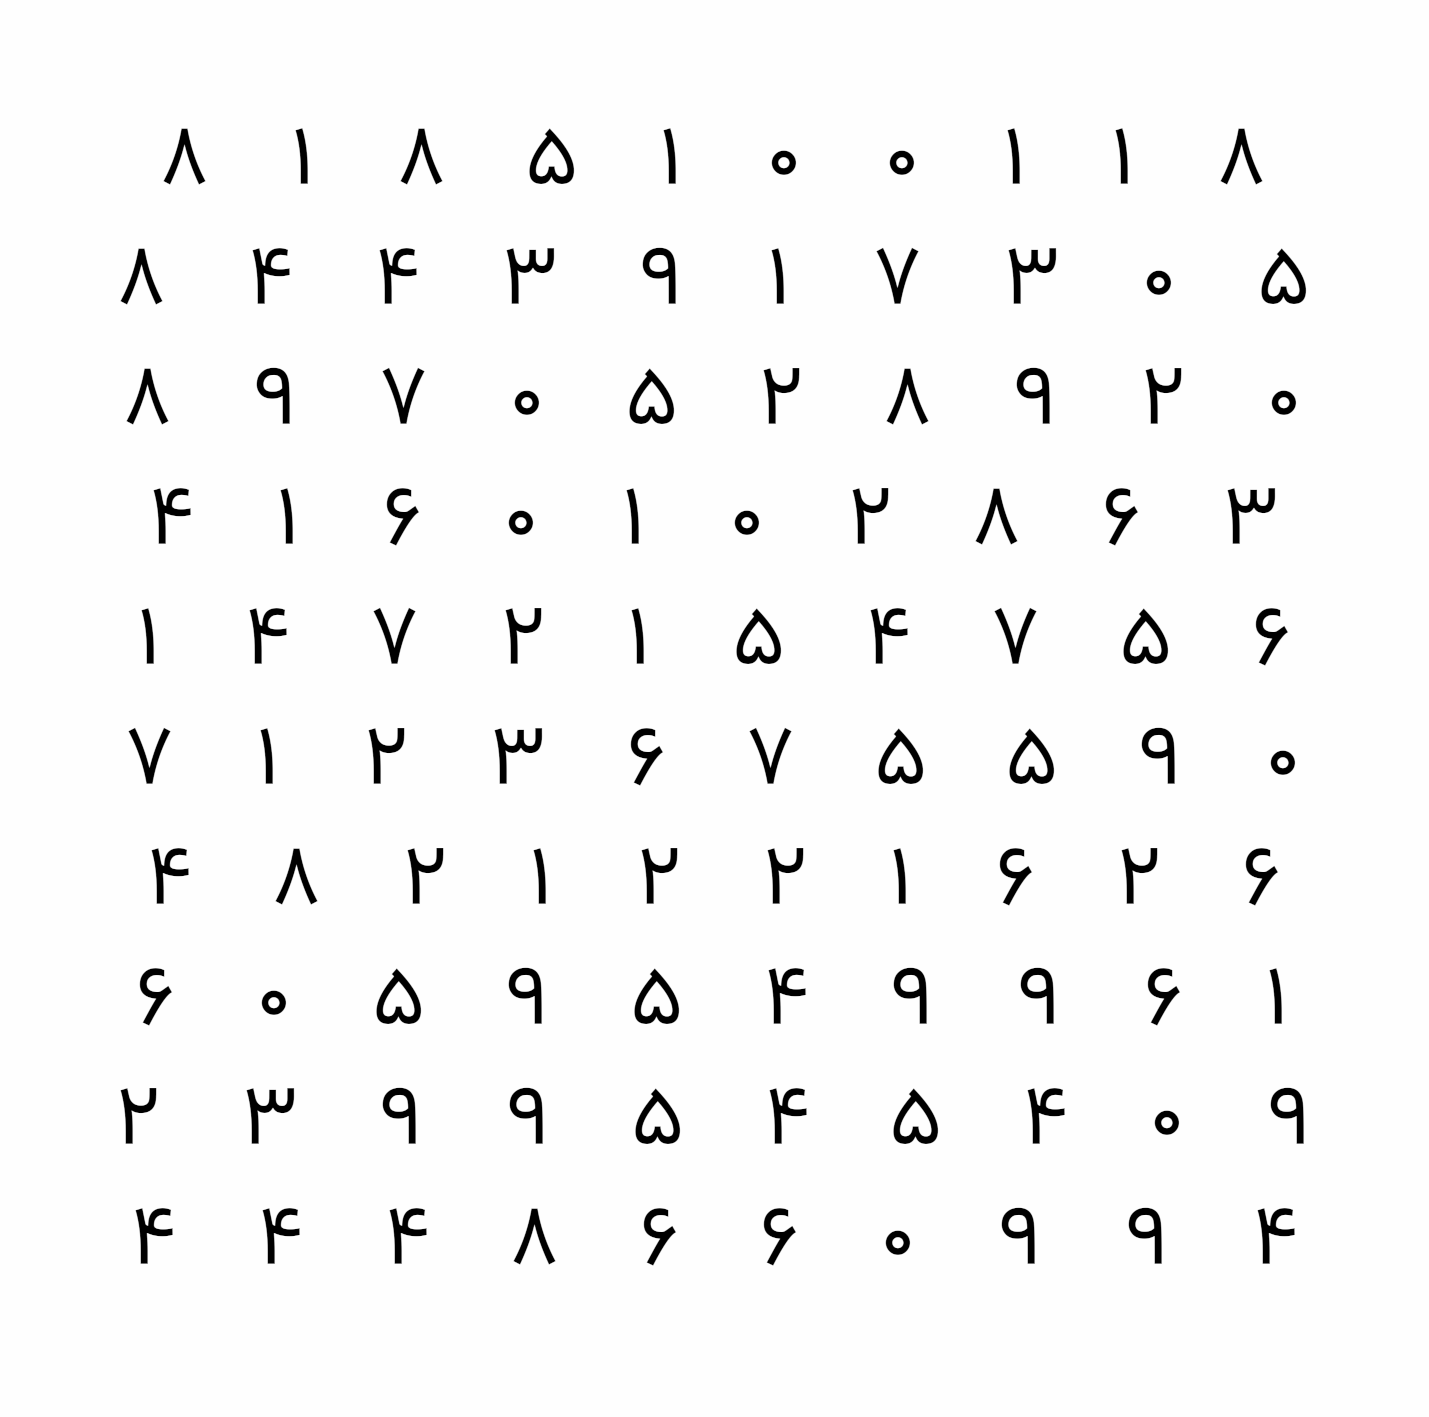
\includegraphics[scale=0.6]{figs/compressed.png}
	\caption{نمونهٔ فایل تولیدشده توسط نگارنده برای تست میزان کمپرس در فرمت PNG}
	\label{example_1}
\end{figure}

\begin{table}
	\centering
	\caption{حجم فایل نمونه در فرمت PNG}
	\label{compare_1}
	\begin{tabular}{@{}ll@{}}
	\toprule
	Size & Format \\ \midrule
	7.7 مگابایت & BMP \\
	98 کیلوبایت & PNG \\ \bottomrule
	\end{tabular}
	\end{table}



\subsection{الگوریتم‌های Lossy}

در این الگوریتم‌ها پس از هر بار فشرده‌سازی مقداری از داده‌ها از دست می‌روند، معیار ارزیابی این الگوریتم‌ها 
مقدار فشرده‌سازی با توجه به میزان هدررفت داده می‌باشد، به علت هدررفت مقداری از داده این الگوریتم‌ها معمولا در 
مواردی که هدررفت اندک داده توسط انسان یا ماشین قابل تشخیص نباشد استفاده می‌شوند،‌ مثلا تکنیک‌های 
ذخیره‌سازی تصاویر و ویدئو‌ها در کامپیوترها مبتنی بر الگوریتم‌های Lossy 
است زیرا چشم انسان قادر به تشخیص عوض شدن تعدادی پیکسل در صفحه پس از بازیابی فایل فشرده‌شده نیست. 

معمولا در فشرده‌سازی Lossy از 
\lr{Transform Coding}
استفاده می‌شود که داده‌ها را از فضای حقیقی به فضایی دیگر(معمولا فرکانس) می‌برد و در آنجا از قسمت‌هایی از داده که تاثیرگذاری و حس‌پذیری کمتری
نسبت به دیگران دارند صرف نظر می‌شود، سپس وارون تبدیل اجرا شده و داده‌های کوچک‌شدهٔ جدید با الگوریتم‌های 
Lossless فشرده می‌شوند. یکی از 
مشهورترین
\lr{Transform Coding} 
ها الگوریتم 
\lr{Discrete Cosine Transform (DCT)}
است که در فصول آتیِ این مستند بیشتر با آن آشنا خواهیم شد. 

\subsubsection{نمونه‌های الگوریتم‌های Lossy}
الگوریتم‌های Lossy با همه‌گیر شدن اینترنت و اشتراک‌گذاری 
بیشتر مدیا در فضای اینترنت بسیار همه‌گیر شدند، از این رو اکثر این الگوریتم‌ها برای فشرده‌سازی فایل‌های صوتی-تصویری یا به اصطلاح 
Media 
استفاده می‌شوند. 

\lr{
\begin{itemize}
	\item JPEG
	\item MP3
	\item MP4
	\item H.26x
\end{itemize}}

به عنوان نمونهٔ برای الگوریتم Lossy 
حالت فشرده‌شدهٔ عکس 
\ref{example_1}
با فرمت JPEG 
با کیفیت‌های مختلف در جدول 
\ref{compare_2}
آورده شده است.
\footnote{در صورتی که تمایل به دیدن اصل فایل‌ها دارید می‌توانید به 
\textit{  \href{https://github.com/merfanian/DataCompressionDoc/LatexFiles/figs/}{Github مستند} 
} 
مراجعه کنید.
} 

\begin{table}[h]
	\centering
	\caption{حجم فایل نمونه در فرمت JPG}
	\label{compare_2}
	\begin{tabular}{@{}lll@{}}
	\toprule
	Quality & Size & Format \\ \midrule
	100 & 7.7 مگابایت & BMP \\
	100 & 98 کیلوبایت & PNG \\
	90 & 96.8 کیلوبایت & JPG \\
	50 & 62.9 کیلوبایت & JPG \\
	20 & 49  کیلوبایت& JPG \\ \bottomrule
	\end{tabular}
	\end{table}



